\chapter{Introduction}
\label{ch:intro}

\section{Mesoscale Convective Systems (MSCs) in the Horn of Africa}

\acrfullpl{mcs} have been shown to account for over 60\% of extreme rainfall in Ethiopia and Somalia \citep{Hill2023}. These events can have devastating impacts on local communities, leading to loss of life, displacement, and significant economic damages. While aggregate data over recent decades is limited, in 2020 alone, nearly 500,000 people were displaced by floods in Ethiopia \citep{Mekuria2022}. Such intense flooding not only affects the local population, but can also impact countries as far as Egypt due to the Ethiopian Highlands being a watershed origin for countless rivers including the Blue Nile \citep{Mamo2019,Legese2020,Zaroug2014}. Projections also show that climate change is likely to alter the frequency and intensity of these storms \citep{Endris2019,Das2016}. Thus, it is important to understand the factors which contribute to the intensification and propagation of \acrshortpl{mcs} in this region.

The Horn of Africa (Figure \ref{fig:horn-of-africa}) has a unique confluence of large-scale climatic variability that affect \acrshort{mcs} development. In contrast to Sub-Saharan West Africa, the \acrfull{itcz} passes over the Horn of Africa twice per year providing the foundation for two distinct rainy seasons \citep{Palmer2023,Tefera2025}. The \acrfull{tej} is a key regional feature enhancing vertical wind shear, which can both facilitate or hinder \acrshort{mcs} development \citep{Farnsworth2011,Vashisht2021}. The \acrfull{mjo} also contributes to intra-seasonal changes in atmospheric conditions. Its active phases coincide with increased convection and extreme rainfall events \citep{Camberlin2019,Ochieng2023,Pohl2006}. Additionally, the \acrfull{enso} and the \acrfull{iod} have also been shown to modulate rainfall patterns in the region \citep{Dubache2019,Endris2019,Vashisht2021,Zaroug2014}. El Niño and positive \acrshort{iod} phases are typically associated with increased rainfall in East Africa, while La Niña and negative \acrshort{iod} phases tend to bring drier conditions \citep{Camberlin2019,Endris2019}.

The region is also geographically diverse, with a range of topographical features that influence local weather patterns. From the west, the Sahel fades into the Ethiopian Highlands and later the East African Rift Valley, characterised by high topographic relief and complex orography. These highlands then transition into the low-lying coastal plains of Somalia. Unlike most other countries at this latitude, most of Somalia is arid or semi-arid, with the exception of its border region with Kenya \citep{Beck2023}. This contrast in geography can be seen in Figure \ref{fig:horn-of-africa} and is reflected in storm development and rainfall patterns. The mountains of Ethiopia dominate local convective processes while the low-lying areas on the south-eastern coast of the region are not nearly as conducive to \acrshort{mcs} development \citep{Negash2024,Camberlin2024}. Thus, the coast is much more susceptible to storm patterns over the Indian Ocean and the Gulf of Aden \citep{Camberlin2024}. The combination of land surface temperature and soil moisture also impact the storm development and intensification. Notably, multiple studies over distinct regions have demonstrated that strong soil moisture gradients can intensify convection \citep{Barton2021,Klein2020,Taylor2017}. These processes are likewise relevant to the Horn of Africa, especially in transitional climates bridging arid and humid zones.

\begin{figure}[ht]
    \centering
    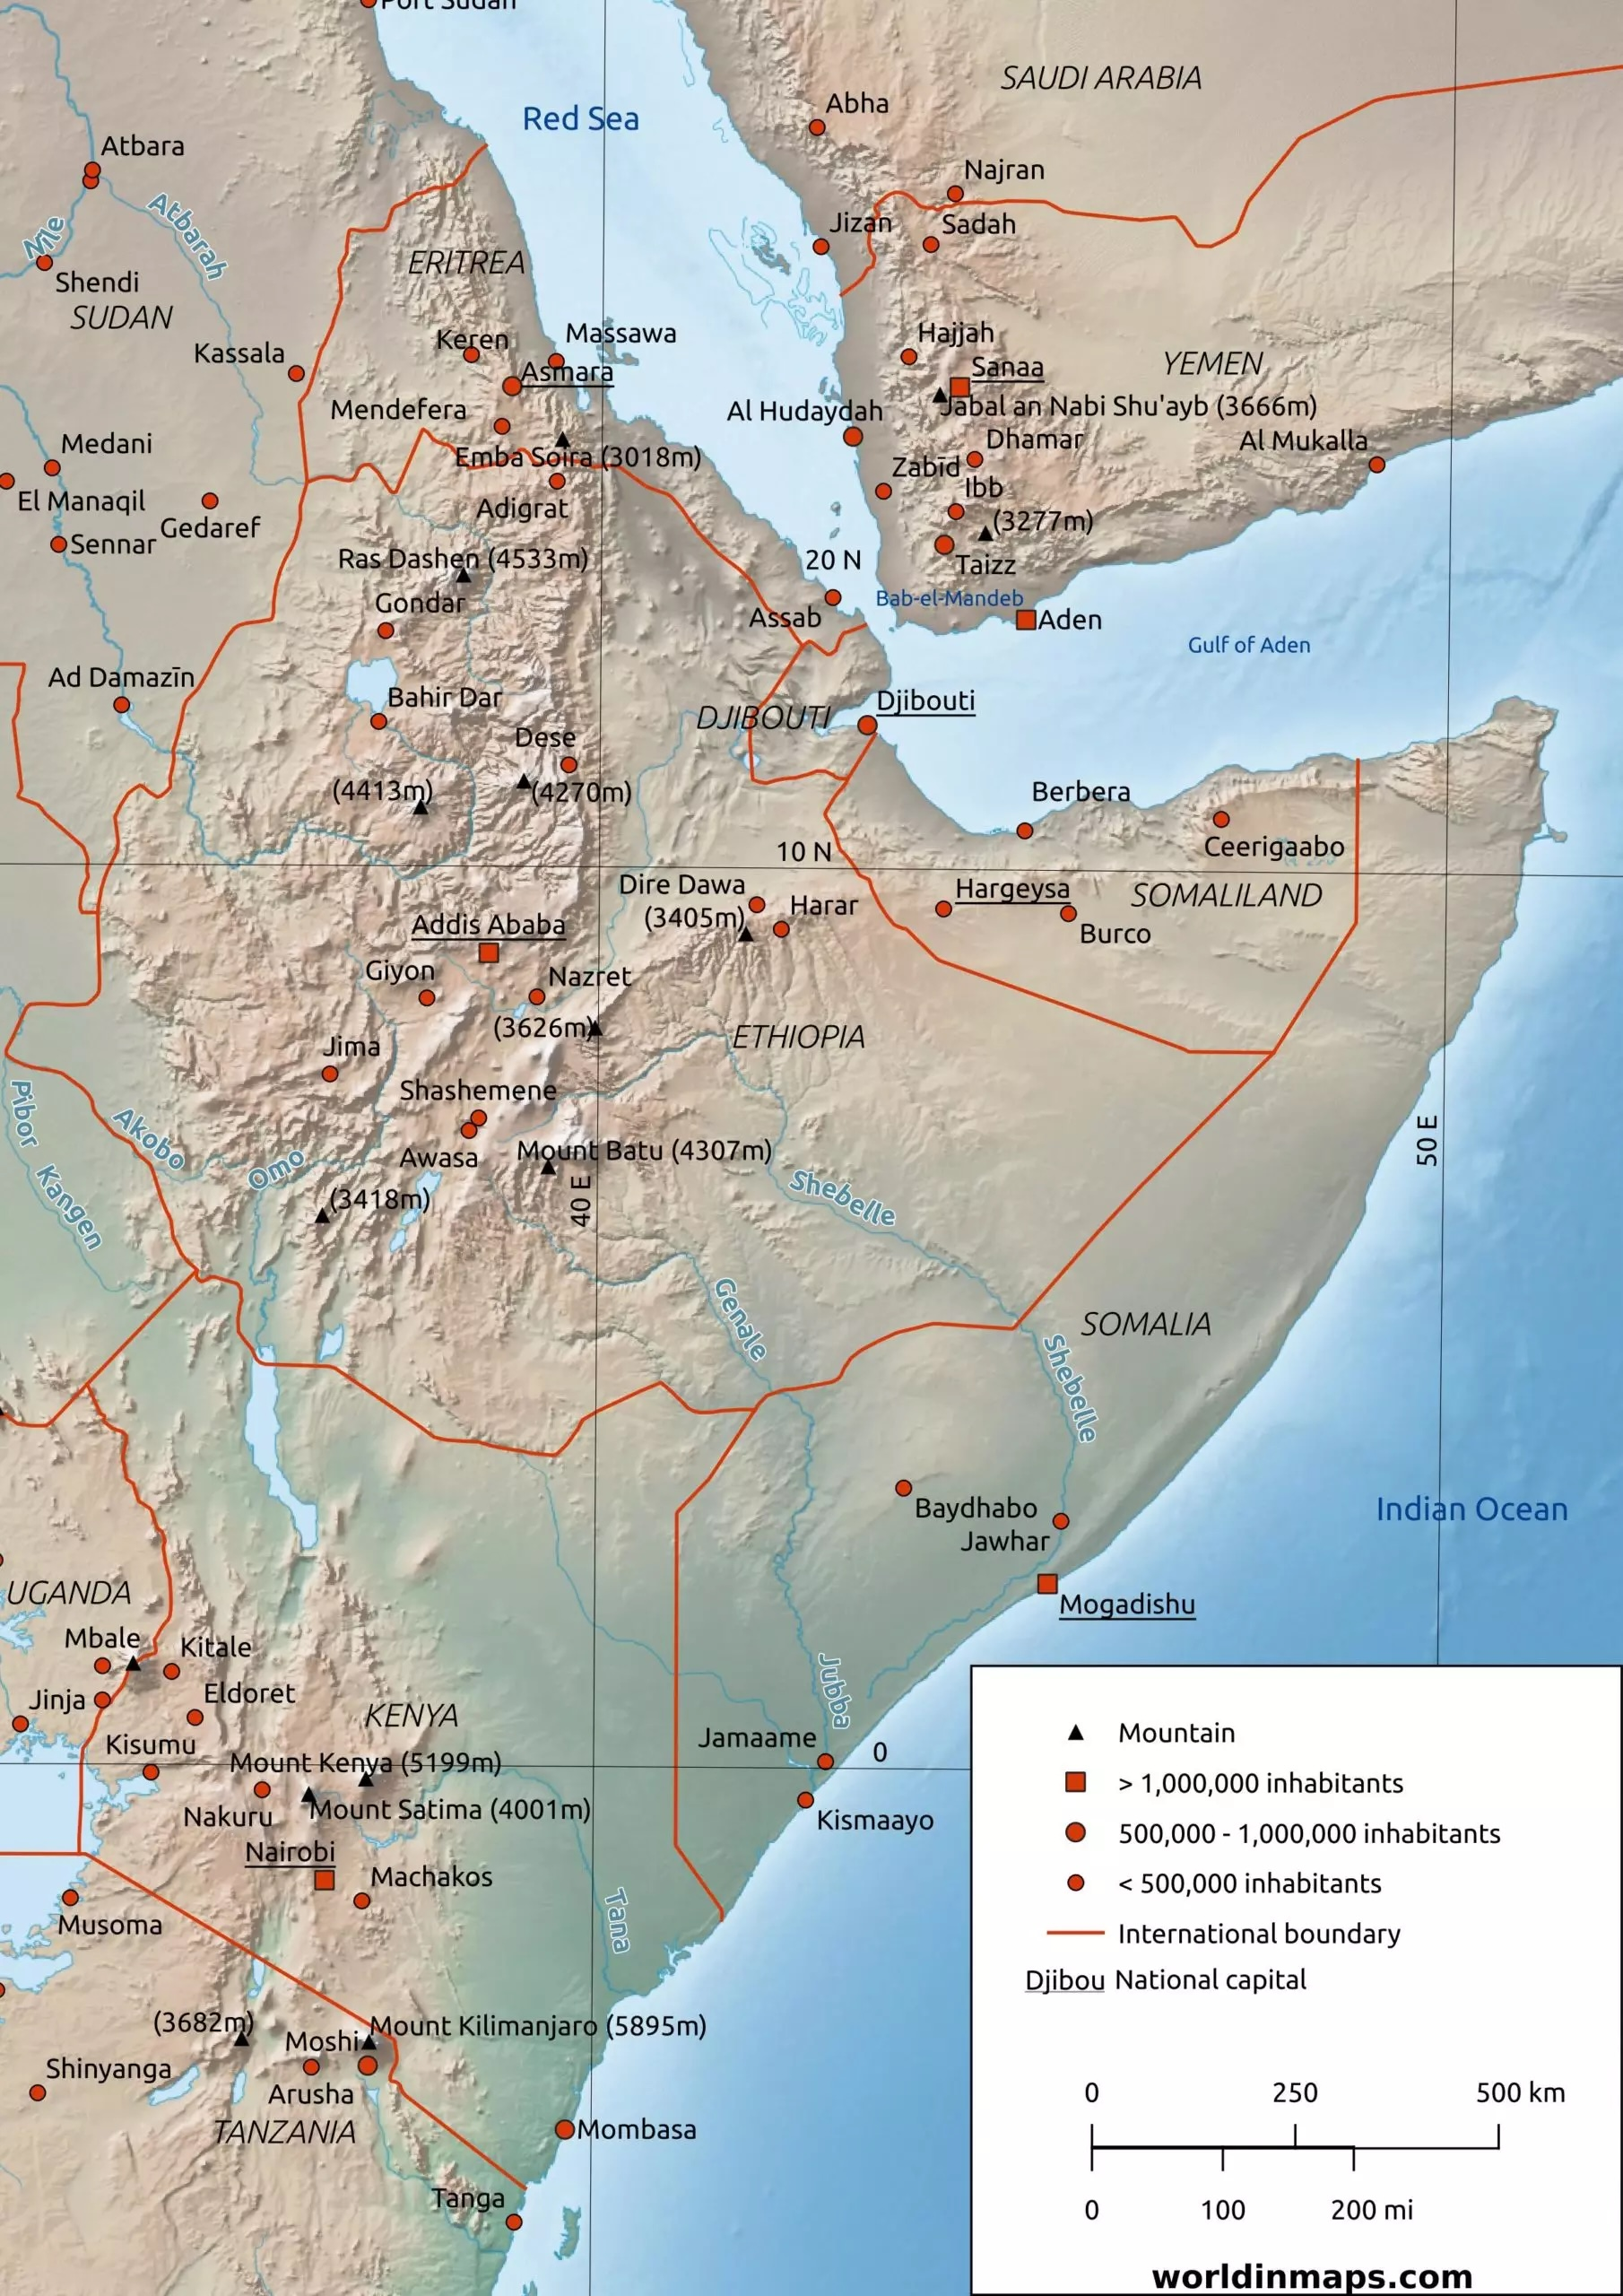
\includegraphics[width=0.6\textwidth]{../figures/static/horn-of-africa-map-scaled.jpeg}
    \caption{Map of the Horn of Africa \citep{WorldInMaps2024}}
    \label{fig:horn-of-africa}
\end{figure}

The primary challenge in rainfall prediction is that \acrfull{nwp} models have historically not operated at high enough resolutions to resolve convective processes and instead use sub-grid parametrisation schemes to more accurately replicate storm behaviour \citep{Stevens2019,Yano2018}. Newer kilometre-scale models are showing promise in more faithfully representing these processes, but large discrepancies still exist between model outputs and observed phenomena. For example, these models tend to underestimate \acrshort{mcs} precipitation totals while overestimating the intensity of precipitation \citep{Feng2025,Stevens2019}. Further complicating the modelling landscape is the mid-latitude bias of many \acrshort{nwp} models, which tend to perform worse in the tropics and subtropics at shorter lead times \citep{Keane2025}. In addition, the entire continent of Africa is considerably under-represented in high-quality meteorological data and many national meteorological services lack critical resources to more effectively monitor and predict \acrshortpl{mcs} \citep{Dinku2019,Kinyondo2018,Meque2021}. This discrepancy also has downstream effects on global meteorology, as reanalysis datasets and digital twin systems rely heavily on data assimilation of observations and regional models for calibration \citep{Linsenmeier2023,Valmassoi2023}. 

Although increased investment and study are undoubtedly necessary, these challenges present an opportunity for innovative methods in the immediate term to make use of existing data to better understand \acrshort{mcs} behaviour. Targeted insights into the factors which contribute to storm intensification and propagation could help inform the design of new observational networks, improve sub-grid parametrisation schemes, and ultimately lead to better forecasts. This is especially imperative in a region like Africa where computational resources are limited, and the need for short-range accuracy is critical. This thesis intends to address said challenges by presenting a reusable framework to identify important factors and quantify their variability.

\section{Explainable Artificial Intelligence (XAI) for Convective Systems}

The field of meteorology has been no exception to the increasing popularity of data-driven methods, with a growing body of literature exploring the application of \acrshort{ml} techniques to various open problems \citep{Bracco2024,Mamalakis2022,Waqas2024}. Ample amounts of manual observations spanning nearly centuries, petabytes of satellite imagery, the output of numerical models and reanalysis datasets like the \acrfull{era5} and \acrfull{merra2} constitute a rich repository of training and validation data \citep{Bracco2024,Waqas2024,Zhang2025}. Given the profound complexity of atmospheric processes, there are numerous opportunities at varying scales to improve our understanding and prediction of weather and climate phenomena. On the smaller scale, \acrshort{ml} has been used for tasks such as downscaling, parametrisation, and nowcasting, where the goal is to improve the resolution and accuracy of existing numerical forecasts \citep{Blunn2024,Zhang2023}. On the larger scale, an especially popular approach known as \acrfull{piml} incorporates constraints directly into the training process to penalise the models for not adhering to the laws of physics \citep{Pathak2022,Luo2025,Zhang2023}.

In spite of the rapid emergence and success of these methods, the fundamental challenge of trustworthiness remains. This is particularly important in domains like meteorology where understanding the rationale behind predictions is crucial \citep{BarredoArrieta2019,Zhang2025}. As a result, there is a growing interest in developing methods for explainable and interpretable \acrshort{ml}, known as \acrfull{xai}, to provide insights into the decision-making processes of these models. There are many such methods including models which are inherently interpretable by design, such as linear regression, as well as post-hoc explanation methods, such as \acrfull{shap}, which can be applied to any model after training \citep{BarredoArrieta2019,Molnar2025}. Unsurprisingly, \acrshort{xai} deployment has also increased across different domains in meteorology, including weather prediction, climate modelling, and extreme event analysis \citep{Mamalakis2022,Yang2024}. More relevant for this thesis, \acrshort{xai} has been employed specifically for understanding convective systems. \cite{Bassine2025} and \cite{Zhang2019} use interpretable models to predict rainfall extremes in Africa and \acrshortpl{mcs} transition into tropical cyclones, respectively. \cite{Zhuo2021} used both \acrshort{piml} and the post-hoc explanation methods to estimate tropical cyclone intensity and size. While these studies span diverse meteorological applications, they underscore the growing potential of \acrshort{xai} for understanding and forecasting convective systems in particular.

The main inspiration for the methodology of this thesis comes from \cite{Hunt2024}'s investigation of interpretable gradient-boosted decision-trees for uncovering dynamical relationships governing \gls{indianmonsoon} \acrfull{lps}. They first utilised a tracking algorithm to assemble a database of \acrshort{lps} storm tracks from \acrshort{era5} data. Using the storm centroids along each track, they extracted a set of meteorological and geographic features from the surrounding \acrshort{era5} data. These features were then used to train a gradient-boosted decision tree model to predict specific storm characteristics, like mean precipitation or peak vorticity. The model was then interpreted using \acrshort{shap} values to not only identify the most important features, but also reveal how feature importance changes relative to geography. Within the results, the authors found that processes affecting intensification differ from those affecting peak intensity and also confirmed existing research that mid-level winds are relevant for predicting storm speed and direction. This methodology is particularly compelling as it also offers a framework that could be adapted for other regions and storm types with the only pre-requisite being high quality storm track data.

However, there are also many additional avenues for exploration, especially leveraging the explanatory power of \acrshort{shap} values. For example, \cite{Hunt2024} primarily focus on the model's ability to capture the relationships between features and storm characteristics, but do not explore the model's ability to predict storm tracks or propagation. While interpretable \acrshort{ml} techniques pale in comparison to traditional \acrfull{nwp} models, their insights may be able to aid with sub-grid parametrisation or facilitate the planning of new observational networks in data-scarce and computationally limited regions like Africa. Furthermore, while \cite{Hunt2024} do take great care to justify the inclusion of each feature and remove those that are highly correlated, they do not explore the possibility of direct comparison between models trained with different feature sets. This could be useful in disentangling the relative importance of meteorological and geographical features, which may often work in concert or direct opposition, such as wind angle and orography. Thus, this thesis aims to build upon their work by exploring these additional avenues and further investigating the potential of interpretable \acrshort{ml} techniques for understanding and predicting storm behaviour.

\section{Research Objectives}

The primary objective of this research is to investigate the factors which contribute to the intensification and propagation of East African \acrfullpl{mcs} through the usage of an interpretable machine learning model and subsequent application of \acrshort{xai} techniques. The methodology will largely follow the framework established by \cite{Hunt2024}, with adaptations made for the specific context of East African storms. A necessary prerequisite for achieving this objective is the creation of a dataset that captures relevant meteorological features along the storm track. This will involve the integration of the East African \acrshort{mcs} database from \cite{Hill2023} with \acrshort{era5} reanalysis data. Next, multiple gradient-boosted decision tree models will be trained to predict various features of storm intensification and propagation using the aforementioned dataset and the \acrfull{xgb} Python library. The choice to use this modelling framework is motivated by its balance between predictive capacity and interpretability, as well as its ability to handle tabular data effectively. The models will be optimised using hyperparameter tuning and their performance compared between similar experiments with different feature sets to assess the impact of feature selection. Finally, \acrshort{xai} techniques, particularly \acrshort{shap}, will be employed to interpret the models' predictions and identify the key factors influencing storm behaviour.

\section{Report Structure}

The main body of this report is organised into 6 chapters with accompanying appendices which contain supplementary material including the full codebase and additional figures. The current chapter, Chapter~\ref{ch:intro}, provides an overview of the research context, objectives, and structure of the report. This includes relevant information on \acrshortpl{mcs} in East Africa, data-driven scientific discovery, \acrfull{xai}, and brief review of current applications of \acrshort{xai} for convective systems. Chapter~\ref{ch:method} will detail all aspects of the research methodology, detailing the East African \acrshort{mcs} database and \acrshort{era5} reanalysis, data processing, feature selection, model training, and the main \acrshort{xai} technique utilised, \acrshort{shap}. Chapter~\ref{ch:results} will present the experimental design and subsequent results. This will entail a comparison of the model performance on different feature sets and an analysis of feature importance using \acrshort{shap} values. This analysis will detail overall feature importance across models and experiments, but also further investigate how feature importance varies over geography and time. Chapter~\ref{ch:discuss} will explore the implications of the findings, limitations, assumptions, and potential for future research. Chapter~\ref{ch:con} concludes the report and summarises the key contributions.